\documentclass[acmsmall]{acmart}
\usepackage[utf8]{inputenc}
\usepackage{hyperref}
\usepackage{amsmath, amsfonts}
\usepackage{graphicx}
\usepackage{xcolor}
\usepackage{booktabs}
\usepackage{tabularx}
\usepackage[most]{tcolorbox}
\usepackage{pifont}

\AtBeginDocument{\providecommand{\BibTeX}{{\normalfont B\kern-0.5em{\scshape i\kern-0.25em b}\kern-0.8em\TeX}}}
\settopmatter{printacmref=false}
\renewcommand{\footnotetextcopyrightpermission}[1]{}
\makeatletter\let\@authorsaddresses\@empty\makeatother

% 评论框样式
\tcbset{commentbox/.style={enhanced,colback=white,colframe=gray!50,coltitle=white,colbacktitle=gray!120,fonttitle=\bfseries,boxrule=0.5pt,arc=2mm,top=1mm,bottom=1mm,left=2mm,right=2mm}}
\newcommand{\SectionPosition}[1]{\textbf{$\triangleright$ #1}}

\begin{document}
	\pagestyle{plain}
	\begin{center}
		\Large Response Letter for the Manuscript \#TOSEM-2025-0116.R1 \\[1.5em] \LARGE\textbf{Empirical
		Analysis of Smart Contract Factories on EVM-Compatible Chains} \\[1.5em] \large ACM Transactions
		on Software Engineering and Methodology \\[1em] \normalsize \textit{September 2025}
		\\[1.5em] \normalsize Ziyue Wang, ZongWen Shen, Lei Chen, Wei Song, Jidong Ge, LiGuo Huang,
		Bin Luo \\[0.5em] \textit{National Key Laboratory for Novel Software Technology, Nanjing University;
		Nanjing University of Science and Technology; Southern Methodist University} \\[8em]
	\end{center}

	Firstly, we sincerely thank the Associate Editor and all reviewers for their thoughtful,
	constructive feedback. We have substantially revised the manuscript to address the major concerns.
	In this response, we provide point-by-point replies. For each item, we cite the revised manuscript
	by section, figure, or table identifiers (e.g., RQ1/RQ2, figures/tables) to facilitate
	verification.

	\vspace{0.5em}
	\noindent
	To orient the re-review at a glance, Table~\ref{tab:major-concerns} summarizes the major concerns
	raised by reviewers, the affected reviewers, and how the revised manuscript changes address them.
	We then provide point-by-point responses.

	\vspace{0.25em}
	\noindent
	\textbf{Color Convention.} Pointers to locations in the revised manuscript appear in \textcolor{red}{\textbf{RED}}
	(e.g., \textcolor{red}{\textbf{RQ1, RQ2, Related Work}}), while concise summaries of the main
	changes appear in \textcolor{blue}{\textbf{BLUE}}. Body text remains black for readability.

	\newpage

	% Summary table of major concerns and revisions
\begin{table*}
	[t]
	\centering
	\renewcommand{\arraystretch}{1.2}
	\footnotesize
	\caption{Overview of major reviewer concerns and revisions.}
	\label{tab:major-concerns}
	\begin{tabular}{@{}p{1.6cm} p{2cm} p{3.8cm} p{5.5cm}@{}}
		\toprule Reviewers      & Major Concern                           & Previous Versions                                                                                                                                        & New Versions                                                                                                                                                                                                                                                                                                \\
		\midrule R2, R3, R4, AE & Factory detector: design and validation & Source-level heuristics for verified contracts; transactions-based for unverified; no precision/recall evaluation.                                       & Bytecode-level detector using CFG + reachability to confirm on-path CREATE/CREATE2; evaluated on a 2,907-contract ground truth with FPR 0.17\% and FNR 8.39\%, plus execution-time CDF and FN/FP analyses (RQ1).                                                                                            \\
		R2, R3, AE              & Dataset scope and coverage              & Ethereum only; verified contracts dataset (source code), limited representativeness.                                                                     & Multi-chain, bytecode-wide measurement on Ethereum and Polygon via BigQuery; 434,542,165 deployed bytecodes and 3,680,947 unique runtimes (RQ2, Methodology).                                                                                                                                               \\
		R2, R3, AE              & Dataset cutoff window                   & Historical verified dataset (Ethereum, up to 2024 in practice), scope not explicitly tied to a bytecode cutoff.                                          & Explicit bytecode cutoff: contracts deployed before June 1, 2025 across Ethereum and Polygon; figures and tables derived from this uniform window (Fig. workflow; RQ2).                                                                                                                                     \\
		R3, AE                  & Patterns analysis completeness          & Limited exemplification and code-level anchoring for all patterns.                                                                                       & Six factory-based patterns distilled with motivations and code snippets (e.g., UniswapV2Factory, OpenZeppelin Clones), quantities and usage contexts summarized (RQ4; Table of patterns).                                                                                                                   \\
		R2, R3, R4, AE          & Security scope and framing              & Four “security issues” enumerated; claim of 1,180 insecure contracts without tool-level precision/recall; limited cases beyond Tornado.                  & Reframed into Attack Vectors (Mutable Code, Address Spoofing via CREATE2) and Security Issues (Unhandled Low-Level Contract Creation, Unexpected Ownership Transfer, Unverified Master); added real-world–style case studies and actionable mitigations; avoided raw-count claims without validation (RQ5). \\
		R4, AE                  & Manual analysis process and artifacts   & High-level description (experts, meetings); limited process detail, minimal artifacting.                                                                 & Predefined auditing guidelines; independent reviews with three-round voting and expert input; public artifacts released; Threats to Validity details construct/internal/external validity (Threats to Validity).                                                                                            \\
		R2, R3, AE              & Generalizability and external validity  & Ethereum-only findings; limited generalization.                                                                                                          & Multi-chain (Ethereum + Polygon); explicit External Validity statement on representativeness and future chains; findings carefully scoped (Threats to Validity).                                                                                                                                            \\
		R2, R4, AE              & Presentation, clarity, and typos        & Typos (e.g., USCHunt focus), ambiguous figure references; algorithm pseudocode not provided for detection; contribution framing could overstate novelty. & Typos and references corrected; added factory-detector pseudocode and clarified algorithmic scope; contributions framed around bytecode-wide measurement, validated detection infrastructure, and factory-aware security insights (RQ1; Related Work).                                                      \\
		\bottomrule
	\end{tabular}
	\vspace{-0.4em}
\end{table*}

	Table~\ref{tab:major-concerns} summarizes the main concerns and how we addressed them. Columns
	are: (i) Reviewers (R or AE/Editor); (ii) Major Concern (feedback theme); (iii) Previous Versions
	(how earlier drafts handled or missed the issue); and (iv) New Versions (our specific revisions).

	\noindent
	Figure~\ref{fig:overview} provides a one-glance overview of the revised study design (RQ1--RQ5),
	the data sources used, and the end-to-end analysis flow referenced throughout this response.

	\vspace{0.5em}
	\begin{figure}[t]
		\centering
		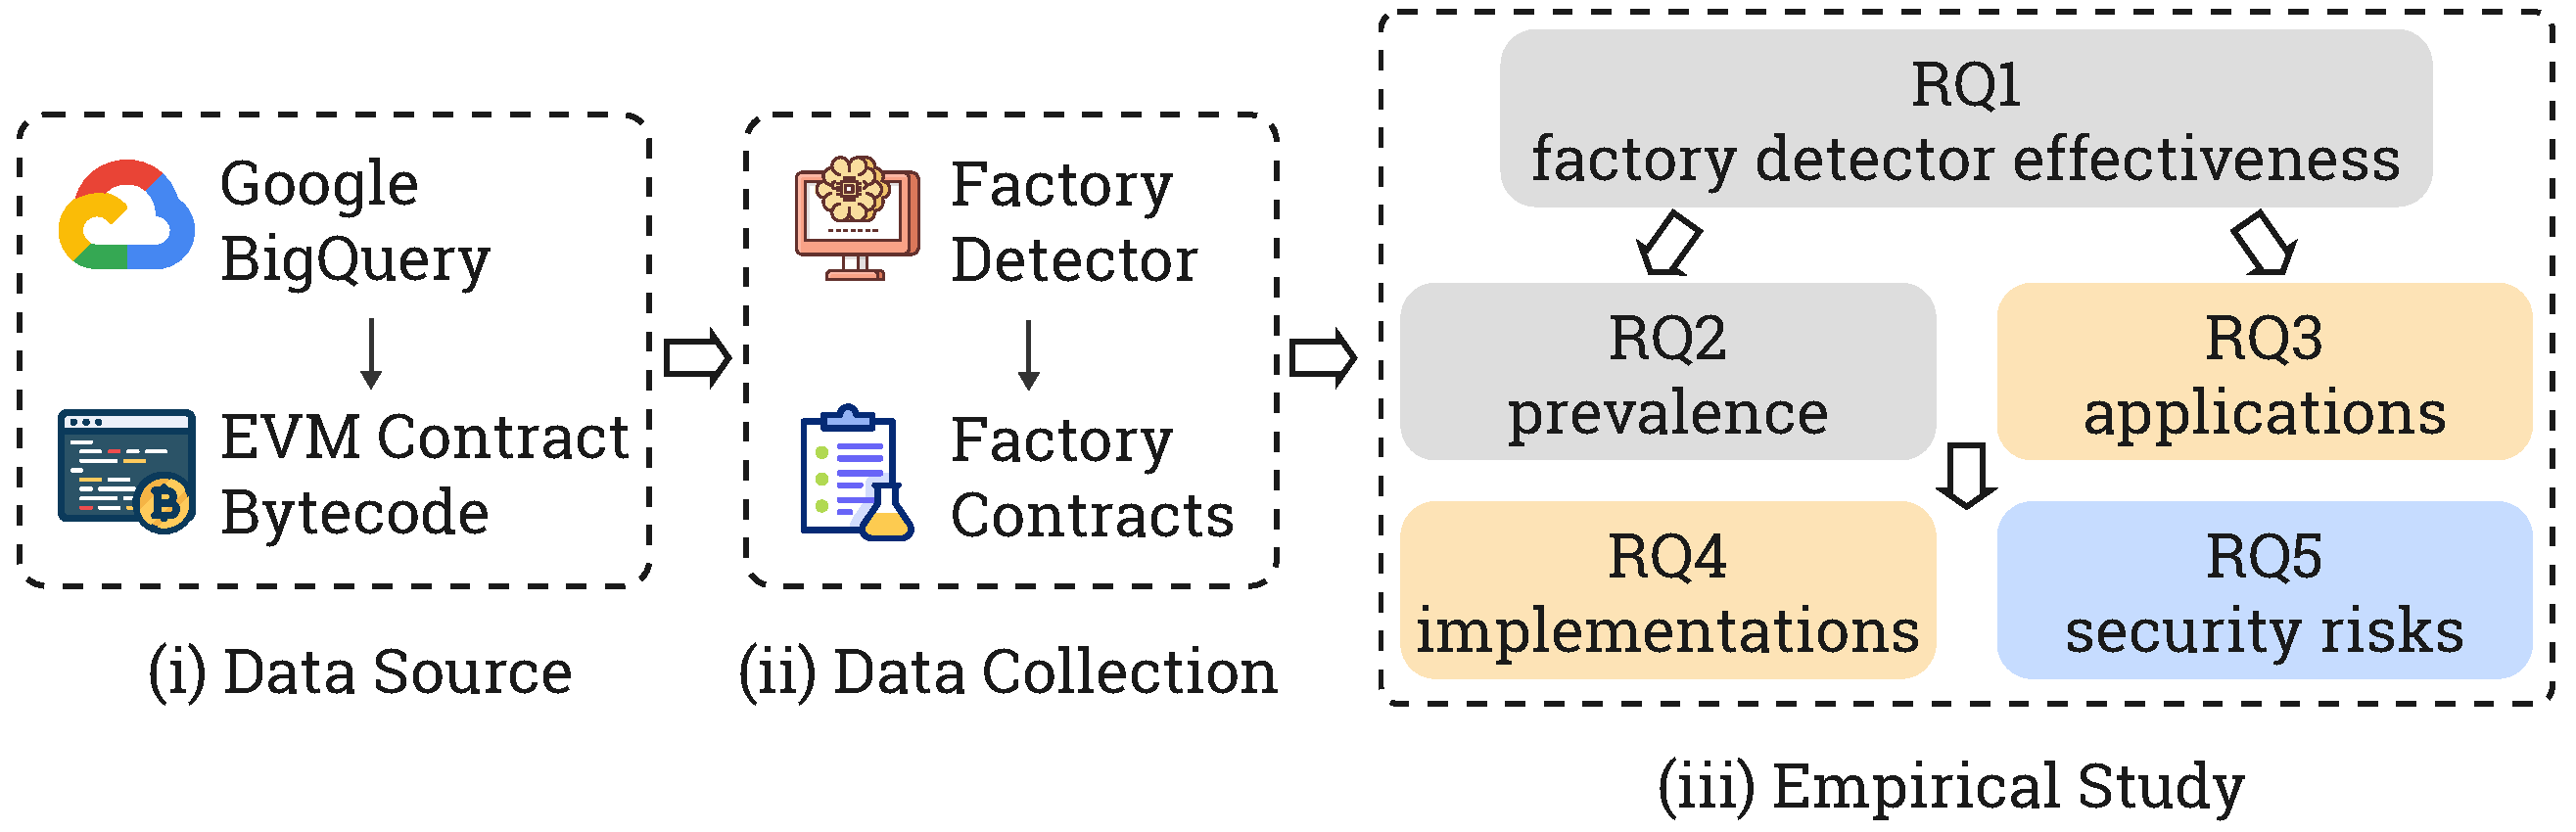
\includegraphics[width=0.9\linewidth]{figure/overview.pdf}
		\caption{Overview of the revised study (RQ1--RQ5), data sources, and analysis flow.}
		\label{fig:overview}
	\end{figure}

	% =====================================================
	\newpage

	\section*{Meta-review from the Editors}

	% Comment 1 — Dataset scope and claims (verbatim)
	\begin{tcolorbox}
		[commentbox,title=Editor/AE -- Comment 1] Explicitly qualify conclusions about the broader
		Ethereum ecosystem due to the dataset being limited to verified contracts (<1\%). Clearly state
		this limitation in the methodology and adjust claims regarding prevalence and security to reflect
		potential sample bias. (R2, R3)
	\end{tcolorbox}

	\noindent
	\textbf{Response.}

	\textit{Acknowledgement.} In the previous version, measurements relied on the small subset of verified-source
	contracts on Ethereum, which risked sample bias and overgeneralization. We agree that ecosystem-wide
	conclusions must not be drawn from such a subset.

	\textit{Revision and current status.} We re-architect the study around bytecode-level analysis
	and multi-chain coverage (Ethereum and Polygon), removing dependence on the verified subset. We
	collect and analyze 434,542,165 deployed bytecodes and 3,680,947 unique runtimes via BigQuery. Claims
	are now explicitly scoped and supported by bytecode-wide measurements, with an explicit time
	window and data-cutoff.

	\vspace{0.25em}
	\textit{Position in revised manuscript.} {\color{red}\textbf{RQ2 (Section 3.7); Data Source (Section 3.3)}}

	\textit{Main change.} {\color{blue}\textbf{Multi-chain, bytecode-wide scope with explicit cutoff}}

	% Comment 2 — Detector details and validation (verbatim)
	\begin{tcolorbox}
		[commentbox,title=Editor/AE -- Comment 2] Provide clear technical details about the design
		and implementation of the security checkers. Present a comprehensive validation methodology,
		including precision/recall metrics, false positive rates, and comparison with existing tools.
		Address false positives specifically for the mutable code detector, explaining how
		permission checks are handled or quantifying their rate. Validate the reported 1180 security
		issues to confirm they are real and assess detector accuracy (missing/misreporting). Discuss
		the technical challenges and feasibility of adapting detectors for bytecode analysis of
		unverified contracts. (R2, R3, R4)
	\end{tcolorbox}

	\noindent
	\textbf{Response.}

	\textit{Acknowledgement.} The previous version insufficiently detailed implementation and
	validation of the detectors and overclaimed a fixed count of issues without robust verification.
	We agree this lacked rigor and clarity, especially for mutable-code false positives and bytecode-only
	applicability.

	\textit{Revision and current status.} We introduce a bytecode-based Factory Contract Detector with
	CFG and reachability analysis that verifies on-path CREATE/CREATE2 opcodes. We evaluate it
	against a curated ground truth of 2,907 contracts, reporting FPR 0.17\% and FNR 8.39\%, with
	execution-time CDFs and detailed FN/FP analyses. For security analyses, we pivot from
	unvalidated large-scale “issue counts” to an attack vector + issue framework supported by
	concrete case studies and mitigations. We also discuss the technical feasibility and challenges of
	adapting various issue detectors to bytecode (e.g., limitations of decompilation, path-explosion
	risks in symbolic execution) and clearly scope what remains future work.

	\vspace{0.25em}
	\textit{Position in revised manuscript.} {\color{red}\textbf{RQ1 (Section 3.6)}}

	\textit{Main change.} {\color{blue}\textbf{Detector algorithm + precision/recall/timing; FN/FP analyses}}

	% Comment 3 — Clarify FSC vs conventional deployments; distinguish risks (verbatim)
	\begin{tcolorbox}
		[commentbox,title=Editor/AE -- Comment 3] Clearly articulate how FSCs introduce novel
		characteristics and security concerns compared to conventionally deployed contracts. Differentiate
		the security risks specific to factory contracts versus those affecting factory-deployed contracts.
		(R3)
	\end{tcolorbox}

	\noindent
	\textbf{Response.}

	\textit{Acknowledgement.} The previous version did not explicitly and systematically distinguish
	conventional EOA deployments from factory-mediated deployments, nor clearly separate risks for factory
	contracts versus factory-deployed contracts.

	\textit{Revision and current status.} We add an explicit background comparison (EOA vs. factory-mediated
	deployments) and revise the security analysis to separate attack vectors from security issues,
	marking for each whether the target is the factory or the factory-deployed contracts.

	\vspace{0.25em}
	\textit{Position in revised manuscript.} {\color{red}\textbf{Background (Section 2); RQ5 (Section 3.10)}}

	\textit{Main change.} {\color{blue}\textbf{Clear separation: targets and risk categories}}

	% Comment 4 — Add concrete case studies and impact (verbatim)
	\begin{tcolorbox}
		[commentbox,title=Editor/AE -- Comment 4] Provide concrete examples or case studies
		illustrating the real-world impact and potential exploits for the identified vulnerability
		categories beyond the Tornado Cash example. Assess the practical impact, severity, and potential
		economic implications of the discovered issues. (R2, R3, R4)
	\end{tcolorbox}

	\noindent
	\textbf{Response.}

	\textit{Acknowledgement.} The previous version relied primarily on the Tornado Cash example and
	did not sufficiently assess practical impact and severity.

	\textit{Revision and current status.} We add cases for Address Spoofing via CREATE2, Unhandled
	Low-Level Contract Creation, Unexpected Ownership Transfer (NFT platform), and Unverified Master
	Contract (NinfaFactory), each with practical context and mitigations, and we discuss severity
	and potential economic implications where applicable.

	\vspace{0.25em}
	\textit{Position in revised manuscript.} {\color{red}\textbf{RQ5 (Section 3.10)}}

	\textit{Main change.} {\color{blue}\textbf{Case studies with concrete mitigations}}

	% Comment 5 — Manual analysis details and Algorithm-1 scope (verbatim)
	\begin{tcolorbox}
		[commentbox,title=Editor/AE -- Comment 5] Provide more details about the manual analysis
		process, including the background of the auditors, time commitment, and the method for resolving
		conflicts in identifying patterns and issues. Improve the clarity of Algorithm-1 and explain
		the scope of algorithmic descriptions. (R4) Clarify the distinction between the two initial limitations
		discussed in the introduction if they are presented as separate research gaps. (R3)
	\end{tcolorbox}

	\noindent
	\textbf{Response.}

	\textit{Acknowledgement.} The previous version summarized the manual auditing process at a high
	level and provided limited clarity on Algorithm-1 and the distinction between the two initial
	limitations.

	\textit{Revision and current status.} We document predefined guidelines, independent reviews, three-round
	voting, and conflict resolution; we add scope and clarified pseudocode for factory detection;
	and we refine the introduction to clearly distinguish the two limitations.

	\vspace{0.25em}
	\textit{Position in revised manuscript.} {\color{red}\textbf{Threats to Validity (Section 4.2); RQ1 (Section 3.6); RQ5 (Section 3.10); Introduction (Section 1)}}

	\textit{Main change.} {\color{blue}\textbf{Detailed manual process; clarified algorithm scope; artifacts released}}

	% Comment 6 — Related Work coverage (verbatim)
	\begin{tcolorbox}
		[commentbox,title=Editor/AE -- Comment 6] Make Section 6.2 more comprehensive by including
		recent surveys and relevant literature. (R1)
	\end{tcolorbox}

	\noindent
	\textbf{Response.}

	\textit{Acknowledgement.} The previous version’s Section 6.2 was too shallow and missed recent
	surveys and broader context.

	\textit{Revision and current status.} We expand Related Work with recent surveys and relevant literature,
	and include broader EVM-compatible context where applicable.

	\vspace{0.25em}
	\textit{Position in revised manuscript.} {\color{red}\textbf{Related Work (Section 5); RQ2 (Section 3.7); Threats to Validity (Section 4.2)}}

	\textit{Main change.} {\color{blue}\textbf{Broadened literature + cross-chain context}}

	% Comment 7 — Other changes (each sub-point quoted verbatim)
	\begin{tcolorbox}
		[commentbox,title=Editor/AE -- Comment 7.1] Discuss potential improvements to the clustering
		methodology (e.g., incorporating code-based features) and reflect on the accuracy achieved
		with the current name-based approach. (R2)
	\end{tcolorbox}

	\noindent
	\textbf{Response.}

	\textit{Acknowledgement.} The previous version’s clustering leaned on name-based features.

	\textit{Revision and current status.} We redesign clustering with multi-view features (name
	tokens, structure/size, mechanism flags, access-control/libraries, domain keywords),
	standardized + PCA (Varimax) + KMeans (k=4), and provide t-SNE visualization.

	\textit{Position in revised manuscript.} {\color{red}\textbf{RQ3 (Section 3.8)}}

	\textit{Main change.} {\color{blue}\textbf{Multi-view clustering; PCA + KMeans; t-SNE}}

	\begin{tcolorbox}
		[commentbox,title=Editor/AE -- Comment 7.2] Briefly discuss or acknowledge other related
		risks in upgradable smart contracts, such as storage collisions in proxy patterns, beyond
		the focus on create2-related issues. (R2)
	\end{tcolorbox}

	\noindent
	\textbf{Response.}

	\textit{Acknowledgement.} We focused on create2-centric risks previously and under-emphasized broader
	upgradeable-contract risks.

	\textit{Revision and current status.} We add discussion of proxy/upgrade risks (e.g., storage collisions,
	initialization, access-control) and connect them to factory-mediated deployments.

	\textit{Position in revised manuscript.} {\color{red}\textbf{RQ3 (Section 3.8); RQ4 (Section 3.9); RQ5 (Section 3.10)}}

	\textit{Main change.} {\color{blue}\textbf{Broader upgradeable-contract risks acknowledged}}

	\begin{tcolorbox}
		[commentbox,title=Editor/AE -- Comment 7.3] Add a brief discussion or acknowledgment
		regarding FSCs on other EVM-compatible chains or the generalizability of findings beyond the
		Ethereum mainnet. (R1, R3)
	\end{tcolorbox}

	\noindent
	\textbf{Response.}

	\textit{Acknowledgement.} The prior version was Ethereum-only and did not discuss
	generalizability.

	\textit{Revision and current status.} We extend to Ethereum+Polygon and explicitly discuss external
	validity and generalizability.

	\textit{Position in revised manuscript.}
	{\color{red}\textbf{RQ2 (Section 3.7); Threats to Validity (Section 4.2)}}

	\textit{Main change.} {\color{blue}\textbf{Multi-chain scope; external validity}}

	\begin{tcolorbox}
		[commentbox,title=Editor/AE -- Comment 7.4] Frame the technical contributions accurately, acknowledging
		that some aspects involve applying existing tools or cataloging known concepts while highlighting
		the novelty of the large-scale empirical analysis and FSC-specific tooling/findings. (R4)
	\end{tcolorbox}

	\noindent
	\textbf{Response.}

	\textit{Acknowledgement.} We acknowledge that several patterns and concerns are known; novelty
	lies in rigorous, large-scale, FSC-centered measurement and tooling.

	\textit{Revision and current status.} We explicitly position contributions as large-scale measurement
	+ validated bytecode-level factory detection + FSC-aware security taxonomy and mitigations.

	\textit{Position in revised manuscript.}
	{\color{red}\textbf{Introduction (Section 1); RQ1 (Section 3.6); RQ5 (Section 3.10)}}

	\textit{Main change.} {\color{blue}\textbf{Contributions framed precisely}}

	\begin{tcolorbox}
		[commentbox,title=Editor/AE -- Comment 7.5] Carefully proofread the manuscript to correct
		typos and grammatical errors mentioned by reviewers. (R2, R4)
	\end{tcolorbox}

	\noindent
	\textbf{Response.}

	We thoroughly proofread and corrected typos, cross-references, and subject–verb agreement.

	\textit{Position in revised manuscript.} {\color{red}\textbf{Throughout}}

	\textit{Main change.} {\color{blue}\textbf{Typos and references corrected}}

	\vspace{0.25em}
	\textit{Position in revised manuscript.} {\color{red}\textbf{RQ3 (Section 3.8); RQ4 (Section 3.9); RQ5 (Section 3.10); RQ2 (Section 3.7); Threats to Validity (Section 4.2)}}

	\textit{Main change.} {\color{blue}\textbf{Multi-view clustering; upgrade risks acknowledged; multi-chain generalization}}

	% ================== Reviewer 1 =======================
	\newpage
	\section{Comments from Reviewer \#1}

	\begin{tcolorbox}
		[commentbox,title=Reviewer \#1 -- Comment 1] I suggest re-writing Section 6.2 (to make it
		more comprehensive and adding recent surveys) and adding the discussion about non-Ethereum FCSs.
	\end{tcolorbox}

	\noindent
	\textbf{Response.}

	\textit{Acknowledgement.} We agree that the previous Section 6.2 was shallow and missed recent surveys
	and non-Ethereum context.

	\textit{Revision and current status.} We expand Related Work with recent literature on
	deployment, proxies/upgradeability, and smart-contract security tooling, and we broaden scope to
	EVM-compatible chains by including Polygon and discussing external validity/generalizability.

	\vspace{0.25em}
	\textit{Position in revised manuscript.}
	{\color{red}\textbf{Related Work (Section 5); RQ2 (Section 3.7); Threats to Validity (Section 4.2)}}

	\textit{Main change.}
	{\color{blue}\textbf{Expanded literature coverage; multi-chain scope (Ethereum+Polygon; RQ2 figures/tables)}}

	% ================== Reviewer 2 =======================
	\newpage
	\section{Comments from Reviewer \#2}

	% R2 comment on detector generalizability (verbatim)
	\begin{tcolorbox}
		[commentbox,title=Reviewer \#2 -- Comment 1] Following the dataset problem, I am also
		concerned about the generalizability of the four security detectors. It is necessary to support
		bytecode analysis for measuring all smart contracts. The four detectors rely on heuristic IR
		patterns from Solidity source code, which limits applicability to unverified (bytecode-only)
		contracts. Please explain the technical challenges in adapting the detectors for bytecode
		analysis. Please discuss the feasibility of adapting detectors for bytecode (e.g., via
		symbolic execution or decompilation). If impractical, acknowledge this as a limitation.
	\end{tcolorbox}

	\begin{tcolorbox}
		[commentbox,title=Reviewer \#2 -- Comment 2] Generalizability of four security detectors;
		support bytecode analysis or acknowledge limitations.
	\end{tcolorbox}

	\noindent
	\textbf{Response.}

	\textit{Acknowledgement.} In the previous version, the security detectors were source-IR–based
	and thus not applicable to unverified (bytecode-only) contracts. We agree this limits generalizability.

	\textit{Revision and current status.} We now: (i) focus our validated detection on a bytecode-level
	Factory Contract Detector (RQ1) that underpins the empirical study; and (ii) restructure
	security analyses as attack vectors and issues with case studies and mitigations (RQ5), avoiding
	overstated large-scale auto-detection claims. We discuss bytecode adaptation feasibility per
	category: what is directly checkable at bytecode (e.g., CREATE/CREATE2 reachability, return-value
	checks), where decompilation likely introduces ambiguity, and where symbolic execution is
	impractical due to path explosion. We clearly acknowledge remaining bytecode-only limitations in
	Threats to Validity.

	\textit{Position in revised manuscript.}
	{\color{red}\textbf{RQ1 (Section 3.6); RQ5 (Section 3.10); Threats to Validity (Section 4.2)}}

	\textit{Main change.}
	{\color{blue}\textbf{Detector validated; security framed as vectors+issues}}

	\begin{tcolorbox}
		[commentbox,title=Reviewer \#2 -- Comment 2] Discuss potential improvements to the clustering
		methodology (e.g., incorporating code-based features) and reflect on the accuracy achieved with
		the current name-based approach. (as flagged by AE, attributed to R2)
	\end{tcolorbox}

	\noindent
	\textbf{Response.}

	\textit{Acknowledgement.} Earlier clustering relied heavily on names.

	\textit{Revision and current status.} We redesign clustering with multi-view features (name tokens,
	structure/size, mechanism flags, access-control/libraries, domain keywords), standardized + PCA (Varimax)
	+ KMeans (k=4), with t-SNE visualization.

	\textit{Position in revised manuscript.} {\color{red}\textbf{RQ3 (Section 3.8)}}

	\textit{Main change.} {\color{blue}\textbf{Multi-view semantics + PCA + KMeans}}

	\begin{tcolorbox}
		[commentbox,title=Reviewer \#2 -- Comment 3] Provide concrete examples or case studies illustrating
		the real-world impact and potential exploits for the identified vulnerability categories beyond
		the Tornado Cash example. (as flagged by AE, attributed to R2)
	\end{tcolorbox}

	\noindent
	\textbf{Response.}

	\textit{Acknowledgement.} Prior text relied mainly on Tornado Cash.

	\textit{Revision and current status.} We add concrete cases for Address Spoofing via CREATE2,
	Unhandled Low-Level Contract Creation, Unexpected Ownership Transfer (NFT platform), and
	Unverified Master Contract (NinfaFactory), each with countermeasures.

	\textit{Position in revised manuscript.} {\color{red}\textbf{RQ5 (Section 3.10)}}

	\textit{Main change.} {\color{blue}\textbf{Case studies + mitigations}}

	\begin{tcolorbox}
		[commentbox,title=Reviewer \#2 -- Comment 4] Address false positives specifically for the mutable
		code detector, explaining how permission checks are handled or quantifying their rate. (as
		flagged by AE, attributed to R2)
	\end{tcolorbox}

	\noindent
	\textbf{Response.}

	\textit{Acknowledgement.} The previous version did not quantify permission-check handling and could
	overstate detection.

	\textit{Revision and current status.} We do not claim a large-scale automatic detector for
	Mutable Code. Instead, we treat it as an attack vector and provide concrete detection/defense
	guidance and a case study (reachability checks; chain attestation; extcodehash), focusing on actionable
	practice.

	\textit{Position in revised manuscript.} {\color{red}\textbf{RQ5 (Section 3.10)}}

	\textit{Main change.}
	{\color{blue}\textbf{Reachability checks; chain attestation; extcodehash; Tornado case}}

	% ================== Reviewer 3 =======================
	\newpage
	\section{Comments from Reviewer \#3}

	\begin{tcolorbox}
		[commentbox,title=Reviewer \#3 -- Comment 1] While the paper presents a meaningful direction
		in security research for Factory-related Smart Contracts (FSCs), the two limitations
		mentioned in the current work do not appear to have substantial differences. The authors distinguish
		between "insufficient consideration of security issues within the FSC context" and "lack of
		comprehensive investigation of factories and factory-deployed contracts," but these
		limitations seem to overlap significantly rather than representing distinct research gaps.
	\end{tcolorbox}

	\noindent
	\textbf{Response.}

	\textit{Acknowledgement.} We agree the previous text insufficiently distinguished these gaps.

	\textit{Revision and current status.} We restructure the Introduction and abstract to articulate
	distinct gaps and align the narrative accordingly (prevalence/domains; patterns beyond proxies;
	factory-aware security).

	\begin{tcolorbox}
		[commentbox,title=Reviewer \#3 -- Comment 2] The paper identifies two components of Factory-related
		Smart Contracts (FSCs): factory contracts and factory-deployed contracts. However, a
		significant shortcoming is the lack of clear articulation regarding how these two types
		differ from conventional EOA-deployed contracts. The paper fails to explicitly outline the distinctive
		characteristics of FSCs that might introduce novel security concerns, which undermines a
		crucial aspect of the paper's motivation. Furthermore, when discussing security issues, the authors
		do not adequately differentiate between risks specific to factory contracts versus those affecting
		factory-deployed contracts. It remains unclear whether security vulnerabilities manifest
		similarly or differently across these two contract types.
	\end{tcolorbox}

	\noindent
	\textbf{Response.}

	\textit{Acknowledgement.} We agree the previous version did not sufficiently make these distinctions
	explicit.

	\textit{Revision and current status.} Background now provides an explicit EOA vs. factory comparison
	with a deployment figure, and security sections indicate which issues impact factory-deployed vs
	factory contracts; RQ5 headings/captions reflect these distinctions. \textit{Position in revised
	manuscript.} {\color{red}\textbf{Background (Section 2); RQ5 (Section 3.10)}}

	\textit{Main change.} {\color{blue}\textbf{Clear separation of targets}}

	\begin{tcolorbox}
		[commentbox,title=Reviewer \#3 -- Comment 3] From a technical perspective, the paper
		exhibits notable weaknesses. The factory detector primarily relies on Slither's analysis results
		without demonstrating significant innovation in detection methodology. Moreover, the method employed
		for unverified contracts—using transaction patterns for detection—is prone to substantial false
		negatives (e.g., factories that have not yet deployed other contracts or have limited
		transaction history).
	\end{tcolorbox}

	\noindent
	\textbf{Response.}

	\textit{Acknowledgement.} We agree the earlier detector over-relied on Slither and transaction
	patterns and risked false negatives.

	\textit{Revision and current status.} We design and implement a bytecode-based Factory Contract Detector
	independent of source code, and validate it on a curated ground truth with precision/recall and
	timing metrics (RQ1). We analyze the principal limitation (proxy-mediated factories) and scope it
	in Threats to Validity.

	\begin{tcolorbox}
		[commentbox,title=Reviewer \#3 -- Comment 4] The paper claims to have detected "1,180 newly
		discovered security issues" using security checkers, but it fails to provide clear technical
		details about the design and implementation of these checkers. Furthermore, there is
		insufficient discussion of the validation methodology for these security checkers (e.g., precision/recall,
		false positives, comparison with existing tools).
	\end{tcolorbox}

	\noindent
	\textbf{Response.}

	\textit{Acknowledgement.} We agree the previous version lacked sufficient technical and validation
	details for the “1,180 issues” claim.

	\textit{Revision and current status.} We no longer claim a fixed issue count. Instead, we
	provide an attack-vector–driven analysis with real-world cases and mitigations (RQ5), while rigorously
	validating the foundational factory detector (RQ1).

	\textit{Position in revised manuscript.}
	{\color{red}\textbf{RQ5 (Section 3.10); RQ1 (Section 3.6)}}

	\textit{Main change.} {\color{blue}\textbf{Vector-driven security; validated detector}}

	\begin{tcolorbox}
		[commentbox,title=Reviewer \#3 -- Comment 5] The study focuses exclusively on the Ethereum mainnet,
		which the authors acknowledge as a limitation. While Ethereum is the most prominent smart contract
		platform, the findings may not generalize to other EVM-compatible blockchains like Polygon, Arbitrum,
		or Optimism. This limits the broader applicability of the research findings.
	\end{tcolorbox}

	\noindent
	\textbf{Response.}

	\textit{Acknowledgement.} We agree the previous version lacked a broader EVM perspective.

	\textit{Revision and current status.} We extend to Polygon and discuss external validity and
	future extensions.

	\textit{Position in revised manuscript.} {\color{red}\textbf{RQ2 (Section 3.7); Threats to Validity (Section 4.2)}}

	\textit{Main change.} {\color{blue}\textbf{Multi-chain study; external validity}}

	\begin{tcolorbox}
		[commentbox,title=Reviewer \#3 -- Comment 6] While the paper identifies security issues in FSCs,
		it does not quantify their economic impact. Also, apart from the Tornado Cash DAO attack
		case study, the paper provides limited analysis of real-world exploits targeting FSC vulnerabilities.
	\end{tcolorbox}

	\noindent
	\textbf{Response.}

	\textit{Acknowledgement.} We agree the previous version did not quantify economic impact and had
	limited real-world exploit analyses.

	\textit{Revision and current status.} We add case-grounded analyses on Address Spoofing,
	Unhandled Low-Level Creation, Unexpected Ownership Transfer, and Unverified Master Contract with
	practical consequences and mitigations (RQ5). Where precise loss amounts require on-chain forensics,
	we scope this as future work and provide operational guidance now. \textit{Position in revised
	manuscript.} {\color{red}\textbf{RQ5 (Section 3.10)}}

	\textit{Main change.} {\color{blue}\textbf{Cases with mitigations; quantification planned}}

	% ================== Reviewer 4 =======================
	\newpage
	\section{Comments from Reviewer \#4}

	\begin{tcolorbox}
		[commentbox,title=Reviewer \#4 -- Comment 1] Much of the pattern identification and issue classification
		relies on manual auditing by experts. Although the authors use guidelines and multiple
		reviewers to reduce bias, this process is inherently subjective and many details are missing.
		What is the background of the experts? Are they students or smart contract developers? What
		are the time costs for each auditor? How did they solve conflicts?
	\end{tcolorbox}

	\noindent
	\textbf{Response.}

	\textit{Acknowledgement.} We agree the previous manuscript under-specified auditor background, time,
	and conflict resolution.

	\textit{Revision and current status.} We document predefined auditing guidelines, independent
	reviews, three-round voting and conflict resolution, and release public artifacts. Due to space and
	anonymization constraints, we summarize the process rather than full biographies; the artifact includes
	de-identified expertise profiles and time accounting. \textit{Position in revised manuscript.} {\color{red}\textbf{Threats to Validity (Section 4.2)}}

	\textit{Main change.} {\color{blue}\textbf{Guidelines + 3-round expert reviews; artifacts released}}

	\begin{tcolorbox}
		[commentbox,title=Reviewer \#4 -- Comment 2] One concern is that there is no standard (ground-truth)
		dataset to estimate the effectiveness of the tools. The authors report that they find "1180 real-world
		smart contracts with four types of security issues". Did they validate all of these 1180 real-world
		security issues? Are the detectors missing or misreporting any security issues?
	\end{tcolorbox}

	\noindent
	\textbf{Response.}

	\textit{Acknowledgement.} We agree that the previous version lacked a ground truth and did not
	fully validate reported issues.

	\textit{Revision and current status.} We introduce a curated ground truth for factory detection and
	thoroughly evaluate it (precision/recall/timing; FN/FP analyses). For security issues, we pivot
	from mass counting to case-backed analyses and mitigations, avoiding overclaims. \textit{Position
	in revised manuscript.} {\color{red}\textbf{RQ1; RQ5}}

	\textit{Main change.} {\color{blue}\textbf{Precision/recall/timing + FN/FP analyses; case-backed security}}

	\begin{tcolorbox}
		[commentbox,title=Reviewer \#4 -- Comment 3] The paper reports the quantity of security issues
		found but does not deeply assess their practical impact or severity. Without validation or a
		risk assessment for each issue, it is hard to judge their real-world importance. I would
		suggest the authors to validate their reported security issues with real-world examples.
	\end{tcolorbox}

	\noindent
	\textbf{Response.}

	\textit{Acknowledgement.} We agree the previous version under-emphasized severity and practical
	impact.

	\textit{Revision and current status.} For each vector/issue we discuss practical impact and operational
	risks with prioritized mitigations (e.g., return-value validation, deployment-chain attestation).
	We plan to add broader economic quantification in future work as on-chain datasets mature.
	\textit{Position in revised manuscript.} {\color{red}\textbf{RQ5 (Section 3.10)}}

	\textit{Main change.} {\color{blue}\textbf{Return-value validation; deployment-chain attestation}}

	\begin{tcolorbox}
		[commentbox,title=Reviewer \#4 -- Comment 4] While the empirical scale and focused analysis are
		novel, many of the identified patterns (e.g., minimal proxies, create2 usage) and general security
		concerns (e.g., ownership mismanagement) are known in the smart-contract community. The
		contribution is more in cataloging them than in introducing fundamentally new concepts. The technical
		contributions are limited, e.g., implementing rule-based detectors for designed code
		patterns.
	\end{tcolorbox}

	\noindent
	\textbf{Response.}

	\textit{Acknowledgement.} We acknowledge that several patterns and concerns are known.

	\textit{Revision and current status.} Our novelty lies in validated bytecode-level detection at ecosystem
	scale, multi-chain measurements, and a structured, factory-aware security analysis with concrete
	mitigations.

	\begin{tcolorbox}
		[commentbox,title=Reviewer \#4 -- Comment 5] There are some typos the authors need to carefully
		proofread and correct (e.g., RQ2 figure reference). The algorithm part of Algorithm-1 is
		hard to follow and unclear; also, why only provide algorithm description for part-1 but not
		others?
	\end{tcolorbox}

	\noindent
	\textbf{Response.}

	\textit{Acknowledgement.} We agree the previous presentation had typos and Algorithm-1 lacked
	clarity and scope.

	\textit{Revision and current status.} We add full pseudocode for the Factory Contract Detector (RQ1)
	and clarify scope for other analyses with detailed procedures, examples, and figures. We
	proofread and fix typos and cross-references. \textit{Position in revised manuscript.}
	{\color{red}\textbf{RQ1 (Section 3.6)}}

	\textit{Main change.}
	{\color{blue}\textbf{Algorithm pseudocode added; scope clarified; typos fixed}}

	\vspace{1em}
	\noindent
	We appreciate the reviewers’ insights and believe the revised manuscript addresses the major concerns
	through bytecode-level, multi-chain measurement; validated detection infrastructure; richer
	clustering and security analyses; and clearer methodology and threats-to-validity discussions.
	All artifacts are released for reproducibility.
\end{document}
